\chapter{La résolution}
\section{Représentation des termes finis}
Nous reprenons ici le très bon formalisme du livre de \textit{Lalement} \cite{lalement}.


Les symboles de constante \verb+true+, \verb+158+, les symboles de fonctions unaires \verb+not+, \verb-+-,
les symboles de fonctions binaires \verb+or+, etc. constituent la signature $\Sigma$ du langage.
Si $f$ est d'arité $n \geq 1$, alors $f$ est un symbole fonctionnel, et si $f$ est d'arité $0$, $f$ est un symbole de constante.
Nous ajoutons à $\Sigma$ un ensemble $X$ de symboles de variables.

L'ensemble des termes $T_{\Sigma \cup X}$ est défini de la manière suivante:
\begin{itemize}
	\item si $c \in \Sigma$ et $c$ d'arité $0$, alors $c \in T_{\Sigma \cup X}$ 
	\item si $f \in \Sigma$ et $f$ d'arité $n \geq  1$ avec $M_1, \dots, M_n \in T_{\Sigma \cup X}$, alors $f M_1 ... M_n \in T_{\Sigma \cup X}$
	\item si $x \in X$, alors $x \in T_{\Sigma \cup X}$
\end{itemize}

Nous pouvons représenter les termes en \textsc{Ocaml} avec le type abstrait suivant:
\begin{Verbatim}
	type terme = 
	| Var of string
	| Func of string * terme list
\end{Verbatim}

En fait, quasiment tous les objets que nous manipulerons pourront être modélisés par des termes.

\vspace{.5cm}
Considérons nos termes préférés : les \textbf{entiers naturels}. 
D'après Kronecker, \textit{God made the integers, all the work is the rest of man}
(traduit ici de l'Allemand par Kleene\cite{meta})


Prenons l'exemple suivant pour définir le \textit{type} des entiers naturels à partir de la signature $\Sigma = \{0, S\}$
Les symboles $O$ et $S$ sont respectivement d'arité $0$ et $1$.
Nous avons ainsi : $$T_\Sigma = \{0, S0, SS0, SSS0, ... \} $$
En \textsc{Ocaml}, nous pourrons écrire:
\begin{Verbatim}
type entiers = Zero | S of entiers 
\end{Verbatim}
En \textsc{Prolog}:
\begin{Verbatim}
entiers(zero).
entiers(s(X)) :- entiers(X)
\end{Verbatim}
En Coq:
\begin{coqdoccode}
\coqdocemptyline
\coqdocnoindent
\coqdockw{Inductive} \coqdocvar{entiers} : \coqdockw{Set} := \coqdocvar{Zero} : \coqdocvar{entiers} \ensuremath{|} \coqdocvar{S} : \coqdocvar{entiers} \ensuremath{\rightarrow} \coqdocvar{entiers} .\coqdoceol
\coqdocemptyline
\coqdocnoindent
\end{coqdoccode}
Les termes se représentent naturellement sous forme d'arbres.

Prenons par exemple le terme \verb+Func("f", [Func("g", [Var "x"; Var "y"]); Var "z"])+
Il sera représenté par l'arbre ci-dessous annoté de ses occurences $u \in \mathcal{O}(M) $ :
\begin{center}
	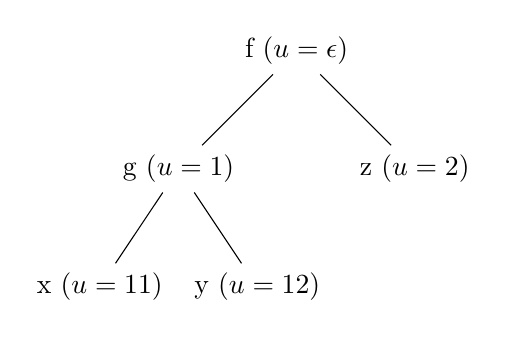
\begin{tikzpicture}[level distance=1.5cm,
	level 1/.style={sibling distance=3cm},
	level 2/.style={sibling distance=2cm}]
	\node{f\ $(u=\epsilon)$}
		child { node {g\ $(u=1)$}
			child { node {x\ $(u=11)$} }
			child { node {y\ $(u=12)$} }
			}
		child { node {z\ $(u=2)$} }
;
\end{tikzpicture}
\end{center}
Pour tout terme $M$, on définit:
\begin{itemize}
	\item L'ensemble $\mathcal{O}(M)$ des occurences de M
	\item Le symbole $M(u)$ en $u$ pour $u \in \mathcal{O}(M)$
	\item Le sous-terme $M|_u$ de $M$ en $u$, pour $u \in \mathcal{O}(M)$
\end{itemize}
Dans le cas où $M = c \in \Sigma$, alors $\mathcal{O}(M) = \{\epsilon\}$, $M(\epsilon)=c$, $M|_\epsilon=c$
 

\vspace{0.5cm}

\noindent Dans le cas où $M = f M_1\dots M_n$, alors :
$$\mathcal{O}(M) = \{\epsilon\} \cup \bigcup_{i=1}^n i. \mathcal{O}(M_i)$$
Avec les égalités suivantes pour les sous-termes $M|_\epsilon = f$ et $M|_{i.u}=M_i|_u $ \\
et de manière équivalente pour les symboles $M(\epsilon) = f$ et $M(i.u)=M_i(u) $

Nous implémentons cela avec un peu de difficulté pour les conversions 
\verb+string+ vers \verb+int+ nécessaire à la manipulation des occurences $u$. 
On considère ici qu'un arbre ne peut avoir plus de 9 fils, donc un seul digit permet de définir le numéro du noeud associé.
\begin{Verbatim}
open String

let rec occurences i terme  =
match terme with
|Var _ | Func(_, []) ->  [i]
|Func (_, m) ->  [i] @ occur_liste 1 i  m 
and occur_liste  c  i lterme =
match lterme with
| [] -> []
| a::b -> (occurences (int_of_string((string_of_int(i)^(string_of_int c)))) a) 
          @ occur_liste (c+1) i b

let reste s =
  if (length s) <= 1 then "0"
  else sub s 1 ((length s) -1)

let string_of_char = String.make 1 ;;

let rec cut i terme =
  match terme with
  | Var _ | Func(_, []) when i=0 -> terme
  | Func(f, lt) -> if i=0 then terme 
                   else subterme (int_of_string(string_of_char((string_of_int i).[0])))
                                 (int_of_string(reste (string_of_int i)))
                                 lt
  | _ -> raise Impossible
and subterme i u ltermes =
  match ltermes with
  | hd::tl -> if (i=1) then  cut u hd else  subterme (i-1) u tl
  | [] -> raise Impossible

\end{Verbatim}
Nous pouvons aussi définir l'opération de \textit{greffe} à une occurence $u$ donnée. Nous utiliserons
l'écriture $M[N]_u$ pour signifier que le terme $M$ reçoit à l'occurence $u$ son greffon $N$.
\begin{Verbatim}
let rec greffe i terme greffon =
match terme with
| Var _ | Func(_, []) when i=0 -> greffon
| Func(f, lt) -> if i=0 then greffon 
				 else Func(f, greffeltermes (int_of_string(string_of_char((string_of_int i).[0]))) 
				  			                (int_of_string(reste (string_of_int i)))  
								            lt
								            greffon)
| _ -> raise Impossible
and greffeltermes i u ltermes greffon =
match ltermes with
| hd::tl -> if (i=1) then  (greffe u hd greffon)::tl  
            else hd::(greffeltermes (i-1) u tl greffon)
| [] -> raise Impossible
\end{Verbatim}

\section{La substitution}
Une substitution est une application $\theta : X \rightarrow T_{X \cup \Sigma} $

Le domaine de substitution est l'ensemble des variables de $X$ telles que $\theta (x) \neq x$
On dit aussi que l'application $\theta$ est l'identité \textit{presque} partout, i.e sauf sur une partie finie
de $X$.
Considérons le domaine de $\theta = \{x_1, ..., x_n\}$, alors $\theta$ est représenté par l'ensemble
des couples (variable, terme) $\{(x_1, \theta (x_1)), ...,(x_n, \theta (x_n) \} $

Nous avons par induction:
\begin{itemize}
	\item $\hat{\theta} c = c$, si $c \in \Sigma$ d'arité 1
	\item $\hat{\theta} (f M_1 \dots M_n) = f(\hat{\theta} M_1 \dots \hat{\theta} M_n )$, si $f \in \Sigma$ d'arité $n$ 
	\item $\hat{\theta} x = \theta (x)$ si $x \in X$
\end{itemize}
La fonction  $\theta$ s'étend ainsi en une fonction $\hat{\theta}$ (mais que nous appelerons aussi $\theta$)
 de  $T_{X \cup \Sigma} \rightarrow T_{X \cup \Sigma} $.
$\hat{\theta}$ est l'unique fonction telle que $\forall x \in X, \hat{\theta}x = \theta (x)$
\begin{center}
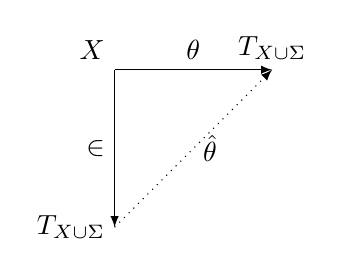
\begin{tikzpicture}[scale=2]
\draw [-latex] (0,0) node[above left]{$X$} -- node[above]{$\theta$} (1,0) node[above]{$T_{X \cup \Sigma} $} ;
\draw  [-latex] (0,0) --node[left]{$\in$} (0,-1) node[left]{$T_{X \cup \Sigma}$} ;
\draw [-latex, dotted] (0,-1) --node[right]{$\hat{\theta}$} (1,0) ;
\end{tikzpicture}
\end{center}

Voici un exemple d'implémentation de la substitution en \textsc{Ocaml}:
\begin{Verbatim}
let valeur_subst sigma var =
  try assoc var sigma
  with Not_found -> var

let rec substituer terme sigma  =
  match terme with
  | Var(x) -> (valeur_subst sigma terme)
  | Func(f, []) -> Func(f, []) 
  | Func(f, args) -> Func(f, (map (function t -> (substituer t sigma)) args))
\end{Verbatim}

\section{Filtrage et réécriture}
\subsection{Le filtrage}
Soient deux termes $M$ et $M'$ appartenant à $T_X$, le filtrage consiste à trouver une substitution $\sigma$
telle que $\sigma M = M'$. Autrement dit, il faut trouver les valeurs à donner aux variables de $M$ pour que celui-ci
soit égal $M'$.

On appelle $M$ le \textit{pattern} et $M'$ l'\textit{instance}.
Nous implémentons cela comme ci-dessous :
\begin{Verbatim}
type terme = 
  | Var of string
  | Func of string * terme list

exception Impossible

let rec filtre_termes lt1 lt2 sigma =
  match (lt1,lt2) with
    | ([], _)  -> sigma
    | (_, []) ->  sigma
    | _ -> 
     begin
	  let sigma1 = filtre (hd(lt1)) (hd(lt2)) sigma in
	  filtre_termes (tl(lt1)) (tl(lt2)) sigma1
    end 
and filtre m n sigma =
  match (m,n) with
	| (Func(f,_), Func(g, _)) when f <> g -> raise Impossible
	| (Var(x), n) -> 
		begin
		try let var_val = assoc (Var(x)) sigma in
			if var_val = n then sigma else raise Impossible
		with Not_found -> (Var(x), n)::sigma
		end 
	| (Func(f,f1), Func(g,g1)) -> filtre_termes f1 g1 sigma 
	| _ -> raise Impossible

let f1 = Func("f", [Var "x"; Func("g", [Var "y"; Var "z"]); Func("h", [Var "x"])]) ;;
let f2 = Func("f", [Func("a",[]); Func("g", [Func("h", [Var "x"]); Func("b", [])]); Func("h", [Func ("a", [])])]) ;;
imprime_sigma (filtre f1 f2 []) ;;
=>>>
z <->  b 
y <-> (h x )
x <->  a 
- : unit = ()
\end{Verbatim}

\subsection{La réécriture et l'arithmétique de Peano}
Le mécanisme de réécriture, très simple à comprendre conceptuellement, est un peu plus difficile
à formaliser proprement.

Un système de \textit{réécriture} est  composé d'une signature $\Sigma$ et d'un ensemble de règles
$\mathcal{R}$ représenté par des couples $(P,Q) \in T_\Sigma [X] \times  T_\Sigma [X]$.

Les couples $(P,Q)$ sont notés $P \longrightarrow Q$

Si nous avons un filtre $\sigma$ tel que $\sigma P = M|_u$, alors le terme $M$ se 
réécrit en un terme $M[\sigma Q]_u$ par l'application de la règle $P \longrightarrow Q$ 
à l'occurence $u \in \mathcal{O}(M)$  
\begin{center}
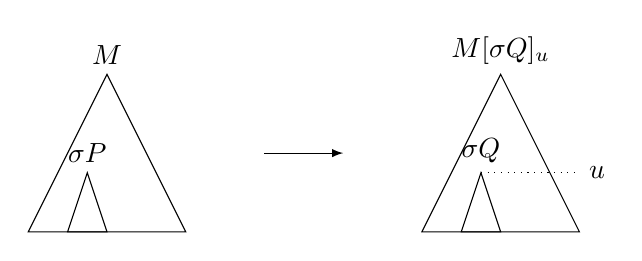
\begin{tikzpicture}
\draw (0,0) -- (2,0) -- (1,2) node[above]{$M$} --cycle ;
\draw (0.5,0) --(1,0)-- (0.75,0.75) node[above]{$\sigma P$} --cycle ;
\draw [-latex] (3,1) --  (4,1) ;
\begin{scope}[xshift=5cm]
\draw (0,0) -- (2,0) -- (1,2) node[above]{$M[\sigma Q]_u$} --cycle ;
\draw (0.5,0) --(1,0)-- (0.75,0.75) node[above]{$\sigma Q$} --cycle ;
\draw [dotted] (0.75,0.75) -- (2,0.75) node[right]{$u$} ; 
\end{scope}
\end{tikzpicture}
\end{center}

\textsc{Ocaml} est <<déjà>> une machine à faire du filtrage et de la réécriture. 
L'application d'une fonction $P$ à son argument $Q$ est modélisé par le redex
$(\lambda m P)Q \longrightarrow \theta P$ où $m$ est le pattern et $\theta$ le filtre de
$m$ vers $Q$, c'est-à-dire $\theta m = Q$.	


Il est ainsi simple de programmer en \textsc{Ocaml} une fonction de réécriture.
Appliquons cela sur l'arithmétique de Peano.

Peano a reconstruit la théorie des
entiers à partir de la fonction successeur. On se donne uniquement le symbole
$S$ d'arité 1 et le symbole de constante 0.
Les entiers sont les termes de la forme $0, S0, SS0, SSS0 \ldots$
Nous pouvons implémenter cela en OCAM avec le type abstrait \verb+peano+
\begin{Verbatim}
type peano = 
	| Zero
	| Succ of peano
	| Plus of peano * peano
	| Mult of peano * peano

let un = Succ Zero ;;
let deux = Succ (Succ Zero) ;;
let trois = Succ (Succ (Succ Zero)) ;;
\end{Verbatim}

Puis nous avons les quatre règles de réécriture suivante:
$$
\begin{array}{ll}
(r_1) & (+\ x\ 0) \rightarrow x \\
(r_2) & (+\  x\ (S\ y)) \to (S\ (+x\ y)) \\
(r_3) & (*\ x\ 0) \to 0 \\
(r_4) & (*\ x\ (S\ y)) \to (+\ y\ (* x\ y)) \\
\end{array}
$$
Ces quatre règles sont implémentées par la fonction \verb+réduire+ ci-dessous:
\begin{Verbatim}
let rec reduire = function
	| Plus (p, Zero) -> reduire p
	| Plus (p1 , (Succ p2)) -> Succ ( reduire ((Plus (reduire p1, reduire p2))) )
	| Mult (p, Zero) -> Zero
	| Mult (p1, (Succ p2)) 
	    -> reduire (Plus (reduire p1, reduire ((Mult (reduire p1, reduire p2))) ))
	| _ as p -> p 

let rec peano_entier = function
	| Zero -> 0
	| Succ p -> 1 + (peano_entier p)
	| any -> peano_entier (reduire any)
	
peano_entier (Plus ( Mult(deux, trois), trois));;
\end{Verbatim}

Essayons maintenant d'implémenter le mécanisme de réécriture en utilisation le type 
\textit{terme} que nous avons précedemment présenté, ainsi que la fonction de filtrage \verb+filtre+ et 
la fonction du substitution \verb+substituer+.

Nous avons fait simple avec cette méthode naïve qui utilise les trois fonctions ci-dessous :
\begin{itemize}
	\item La première \verb+rewrite+ utilise la fonction \verb+filtre+ pour chercher une substitution
	égalisant notre terme avec la partie gauche de la règle de substitution. Si cette substitution est trouveée, la 
	fonction retourne la partie droite de la règle appliquée à la substitution. Dans le cas contraire, la fonction
	est appelée récursivement sur l'ensemble des arguments du terme.
	\item  La seconde \verb+rewriteall+ déroule l'ensemble des règles représentées par une liste de paires $(l,r)$ tant
	que la réécriture ne modifie par le terme.
	\item La troisième \verb+rewrite_bourrin+ itère la fonction précédente tant que l'on peut réduire le terme.
	Désolé pour cette méthode bourrin, mais ça fonctionne\dots
\end{itemize}

\begin{Verbatim}
let rec rewrite t l r =
match t with
| Var(_) | Func(_,[]) -> t
| Func(f, listet)  -> 
	try let subst = filtre l t [] in
		substituer r subst 
	with Impossible -> Func(f, map (function t -> (rewrite t l r)) listet)
and rewriteall lregles t =
	match lregles with
	| [] -> t
	| (l,r) ::reste -> 
		let t1 = (rewrite t l r) in
			if t1=t then rewriteall reste t 
			else t1
and rewrite_bourrin t lregles =
	let t1 = rewriteall lregles t in
	if t1=t then t
	else rewrite_bourrin t1 lregles
\end{Verbatim}

Les quatre règles de Peano sont modélisées de la façon suivante :
\begin{Verbatim}
let peano = [
(Func("+", [Var "x"; Func("0", [])]), Var "x") ;
(Func("+", [Var "x"; Func("S", [Var "y"])])), Func("S", [Func("+", [Var "x"; Var "y"])]) ;
(Func("*", [Var "x"; Func("0", [])]), Func("0", [])) ;
(Func("*", [Var "x"; Func("S", [Var "y"])])), Func("+", [Var "x"; Func("*", [Var "x"; Var "y"])]) ;
] 
\end{Verbatim}

Nous pouvons ainsi calculer la valeur 16 :
\begin{Verbatim}
let un = Func("S", [Func("0", [])]) ;;
let deux = Func("+", [un; un]) ;;
let quatre = Func("*", [deux;deux]) ;;
let seize = Func("*", [quatre;quatre]) ;;

rewrite_bourrin seize peano ;;    
	
\end{Verbatim}



\section{L'unification des termes}
Un interprète PROLOG peut être considéré comme une machine à unifier.

Définissons d'abord l'opération d'unification de deux termes.
Un unificateur de deux termes $t_1$ et $t_2$ est une substitution $\sigma$ telle que $\sigma t_1 = \sigma t_2$

Soit $E$, un système d'équations, on peut définir des transformations $E_{1} \rightarrow _t   E_{2} $
entre systèmes d'équations. On note le symbole $\bot$ qui représente un système sans solution.
Résoudre $E_0$ consiste à appliquer une suite de transformations $E_{0} \rightarrow _*   E_{n} $ de sorte que
$E_{n}$ soit en forme résolue, ou bien $E_{n} = \bot$

Nous avons six types de transformations possibles: 


\begin{tabular}{ll}
décomposition & $E \cup \{ f M_1 \dots M_r = f N_1 \dots N_r \} \rightarrow   E \cup \{ M_1 = N_1 , \dots ,M_r = N_r \} $ \\ 
effacement & $E \cup \{ M=M \} \rightarrow   E $ \\ 
élimination & $E \cup \{ x=M \} \rightarrow  E[x:=M] \cup \{ x=M \}$  si $M \notin X, x \notin var(M)$\\ 
inversion & $E \cup \{ M=x \}  \rightarrow  E \cup \{ x=M \}$ si $M \notin X$ \\ 
conflit &  $E \cup \{ f M = g M\} \rightarrow   \bot $ si $ f \neq g $  \\ 
cycle & $E \cup \{ x=M \} \rightarrow  \bot $ si $x \in var(M)$ \\ 
\end{tabular}

\vspace{0.5cm}

La difficulté de cet algorithme est  sa condition d'arrêt. 
 Si aucune règle ne peut plus s'appliquer sur les éléments du système d'équations, alors l'algorithme doit s'arrêter et son résultat est
la substitution unifiant les deux termes initiaux.
Avec une seule fonction parcourant le système d'équations, représentés en \textsc{Ocaml} par le type \verb+(term * term) list+,
je pense que ce n'est pas possible. Je me suis là aussi un peu cassé les cheveux.
Voici mon code avec deux fonctions:
\begin{Verbatim}
let rec  unifier equation =
match equation with
| (Var(x),Var(y)) -> if x=y then [] else [(Var(x), Var(y))] 
| (Func(f1,l1),Func(f2, l2)) -> if f1 = f2 && List.length l1 = List.length l2 
	then unifierliste (List.combine l1 l2)
	else raise Impossible
| (Func(m,n),Var(x)) -> unifier (Var(x), Func(m,n)) 
| (Var(x), Func(m,n)) -> if (mem (Var(x)) (listevar (Func(m,n)))) 
	then raise Impossible
	else [(Var(x), Func(m,n)) ] 
and unifierliste = function
| [] -> []
| (x,y)::t ->
	let t2 = unifierliste t in
	let t1 = unifier ((substituer x t2 ),(substituer y t2)) in
	t1 @ t2
\end{Verbatim}
% 

On retrouve dans la fonction \verb+unifier+, qui travaille uniquement sur une paire de terme, les différentes règles
de l'algorithme. La fonction \verb+unifierliste+ va unifier sa première paire en utilisant la substitution trouvée dans le reste
de l'équation. C'est un bel exemple de récursivité qui nous dépasse très souvent... 
Ce bout de code vient du site de l'université de Cornell.

Voici un autre exemple moins proche de l'algorithme présenté.
\begin{Verbatim}
let unifier t1 t2 =
  let rec unificateur t1 t2 =
    match (t1,t2) with
    | (Var(x), _)  -> 
      begin
        if t1 = t2 then [] 
        else if (mem t1 (listevar t2)) then raise Impossible
             else [(t1, t2)]
      end		  
    | (_, Var(x)) -> unificateur t2 t1
    | (Func(x, l1), Func(y, l2)) -> if x<>y then raise Impossible
      else (unifliste l1 l2 [])
  and unifliste l1 l2 sigma =
    match (l1, l2) with
    | ([], _) -> sigma
    | (h1::t1, h2::t2) ->
      begin
        let sigma1 = (unificateur h1 h2) in
        unifliste (map (function terme -> (substituer terme sigma1)) t1)
          (map (function terme -> (substituer terme sigma1)) t2)
          (compose_subst sigma sigma1)
      end		
    | _ -> raise Impossible
  in unificateur t1 t2 
\end{Verbatim}


\section{Un mini \textsc{Prolog}}
\begin{Verbatim}
let question() =
	begin
	  print_string "\n autre solution 1/2 (1=oui, 2=non) ? :" ;
	  if read_int()= 1  then false else true 
	end
  
let autre_solution lvar lvaleur  =
	if lvaleur <> [] then (affiche_solution lvar lvaleur ; question())
	else false 
  
let prolog but lregles =
	let lvar_but = listevar but in
	let rec prouveli lbuts lvaleur =
	  match lbuts with
	  | [] -> autre_solution lvar_but lvaleur
	  | h::t -> 
		some (fun regle ->  try
				 let regle_bis = (renomme regle) in
				 let sigma1 = unifier h (hd regle_bis) in			
				 prouveli 
				   (sublis sigma1 ((lhypotheses regle_bis) @ t))
				   (sublis sigma1 lvaleur)  
			   with Impossible -> false)
		  lregles 
	in
	prouveli [but] lvar_but
  
\end{Verbatim}

\section{Quelques exemples de programmation en \textsc{Prolog}}
\subsection{Les entiers naturels}
Définissons en PROLOG le type des entiers naturels avec la fonction \verb+nat+ d'arité 1, la fonction \verb+s+
d'arité 1 et la constante \verb+0+.
Nous avons ainsi les 2 règles:
$$
\begin{array}{l}
nat(0) \Leftarrow \\
nat(s(x)) \Leftarrow nat(x)
\end{array}
$$
\begin{Verbatim}
---------------------------------------------------
let nat = [ [Func("nat", [Func("0", [])])] ;
            [Func("nat", [Func("s",[Var("X")])]) ; Func("nat", [Var("X")])] ] ;;
let but = Func("nat", [Var("X")]) ;; 

prolog but nat ;;
----------------------------------------------------
vincent@HP-Notebook:~/workspace vscodium$ ./prolog.byte 
 X  <->  0 
 autre solution 1/2 (1=oui, 2=non) ? :1
 X  <-> (s 0 )
 autre solution 1/2 (1=oui, 2=non) ? :1
 X  <-> (s(s 0 ))
 autre solution 1/2 (1=oui, 2=non) ? :1
 X  <-> (s(s(s 0 )))
 autre solution 1/2 (1=oui, 2=non) ? :2
vincent@HP-Notebook:~/workspace vscodium$ 
\end{Verbatim}

\subsection{Les additions de Peano}
Nous pouvons modéliser les additions avec l'arithmétique de Peano en utilisant les deux propositions suivantes:
$$
\begin{array}{l}
	add(x, 0, x) \Leftarrow \\
	add(x, s(y), s(z)) \Leftarrow  add(x,y,z)
\end{array}
$$
Puis demandons à notre mini Prolog de résoudre l'équation $add(x,y, s(s(s(0))))$
\begin{Verbatim}
(* les entiers de peano *)
let peano = [ [Func("add", [Var("x"); Func("0", []); Var("x")]) ] ;
				[Func("add", [Var("x");  Func("S", [Var("y")]) ; Func("S", [Var("z")])]) ;
				Func("add", [Var("x"); Var("y"); Var("z")])]
			] ;;

let but1 = Func("add", [Var("x") ; Var("y") ; Func("S", [Func("S", [Func("S", [Func("0", [])])])])]) ;; 

vincent@HP-Notebook:~/vsc$ ./prolog.byte 
 x  <-> (S(S(S 0 ))) y  <->  0 
 autre solution 1/2 (1=oui, 2=non) ? :1
 x  <-> (S(S 0 )) y  <-> (S 0 )
 autre solution 1/2 (1=oui, 2=non) ? :1
 x  <-> (S 0 ) y  <-> (S(S 0 ))
 autre solution 1/2 (1=oui, 2=non) ? :1
 x  <->  0  y  <-> (S(S(S 0 )))
 autre solution 1/2 (1=oui, 2=non) ? :1
vincent@HP-Notebook:~/vsc$ 
\end{Verbatim}
\subsection{Programmation "logique" en \textsc{Coq}}
L'utilisation des types dépendants en \textsc{Coq} nous permet également de définir
les relations \textsc{Prolog}.
\begin{coqdoccode}
	
\coqdocemptyline
\coqdocnoindent
\coqdockw{Inductive} \coqdocvar{entier} :=\coqdoceol
\coqdocnoindent
\ensuremath{|} \coqdocvar{O}: \coqdocvar{entier}\coqdoceol
\coqdocnoindent
\ensuremath{|} \coqdocvar{S}: \coqdocvar{entier} \ensuremath{\rightarrow} \coqdocvar{entier}.\coqdoceol
\coqdocemptyline
\coqdocnoindent
\coqdockw{Fixpoint} \coqdocvar{somme} (\coqdocvar{e1} \coqdocvar{e2}:\coqdocvar{entier}):\coqdocvar{entier} :=\coqdoceol
\coqdocindent{1.00em}
\coqdockw{match} \coqdocvar{e1} \coqdockw{with}\coqdoceol
\coqdocindent{1.00em}
\ensuremath{|} \coqdocvar{O} \ensuremath{\Rightarrow} \coqdocvar{e2}\coqdoceol
\coqdocindent{1.00em}
\ensuremath{|} \coqdocvar{S} \coqdocvar{e1} \ensuremath{\Rightarrow} \coqdocvar{S} (\coqdocvar{somme} \coqdocvar{e1} \coqdocvar{e2})\coqdoceol
\coqdocindent{1.00em}
\coqdockw{end}.\coqdoceol
\coqdocemptyline
\coqdocnoindent
\coqdockw{Lemma} \coqdocvar{somme\_O} : \coqdockw{\ensuremath{\forall}} \coqdocvar{e}:\coqdocvar{entier}, \coqdocvar{somme} \coqdocvar{e} \coqdocvar{O} = \coqdocvar{e}.\coqdoceol
\coqdocnoindent
\coqdockw{Proof}.\coqdoceol
\coqdocindent{4.00em}
\coqdoctac{intro} \coqdocvar{e}.\coqdoceol
\coqdocindent{4.00em}
\coqdoctac{induction} \coqdocvar{e}.\coqdoceol
\coqdocindent{4.00em}
\coqdoctac{simpl}. \coqdoctac{reflexivity}.\coqdoceol
\coqdocindent{4.00em}
\coqdoctac{simpl}. \coqdoctac{rewrite} \coqdocvar{IHe}. \coqdoctac{reflexivity}.\coqdoceol
\coqdocnoindent
\coqdockw{Qed}.\coqdoceol
\coqdocemptyline
\coqdocnoindent
\coqdockw{Lemma} \coqdocvar{somme\_S} : \coqdockw{\ensuremath{\forall}} (\coqdocvar{e1} \coqdocvar{e2}:\coqdocvar{entier}), \coqdocvar{somme} \coqdocvar{e1} (\coqdocvar{S} \coqdocvar{e2})= \coqdocvar{S} (\coqdocvar{somme} \coqdocvar{e1} \coqdocvar{e2}).\coqdoceol
\coqdocnoindent
\coqdockw{Proof}.\coqdoceol
\coqdocindent{4.00em}
\coqdoctac{intros}.\coqdoceol
\coqdocindent{4.00em}
\coqdoctac{induction} \coqdocvar{e1}. \coqdoctac{simpl}. \coqdoctac{reflexivity}.\coqdoceol
\coqdocindent{4.00em}
\coqdoctac{simpl}.\coqdoceol
\coqdocindent{4.00em}
\coqdoctac{rewrite} \coqdocvar{IHe1}. \coqdoctac{reflexivity}.\coqdoceol
\coqdocnoindent
\coqdockw{Qed}.\coqdoceol
\coqdocemptyline
\coqdocnoindent
\coqdockw{Compute} \coqdocvar{somme} (\coqdocvar{S} \coqdocvar{O}) (\coqdocvar{S} \coqdocvar{O}).\coqdoceol
\coqdocemptyline
\coqdocnoindent
\coqdockw{Inductive} \coqdocvar{sommeProlog} : \coqdocvar{entier} \ensuremath{\rightarrow} \coqdocvar{entier} \ensuremath{\rightarrow} \coqdocvar{entier} \ensuremath{\rightarrow} \coqdockw{Prop} :=\coqdoceol
\coqdocnoindent
\ensuremath{|} \coqdocvar{SommeO}: \coqdockw{\ensuremath{\forall}} \coqdocvar{x}, \coqdocvar{sommeProlog} \coqdocvar{x} \coqdocvar{O} \coqdocvar{x}\coqdoceol
\coqdocnoindent
\ensuremath{|} \coqdocvar{SommeS}: \coqdockw{\ensuremath{\forall}} \coqdocvar{x} \coqdocvar{y} \coqdocvar{z}, \coqdocvar{sommeProlog} \coqdocvar{x} \coqdocvar{y} \coqdocvar{z} \ensuremath{\rightarrow} \coqdocvar{sommeProlog} \coqdocvar{x} (\coqdocvar{S} \coqdocvar{y}) (\coqdocvar{S} \coqdocvar{z}).\coqdoceol
\coqdocemptyline
\coqdocnoindent
\coqdockw{Example} \coqdocvar{un\_plus\_un} : \coqdocvar{sommeProlog} (\coqdocvar{S} \coqdocvar{O}) (\coqdocvar{S} \coqdocvar{O}) (\coqdocvar{S} (\coqdocvar{S} \coqdocvar{O})).\coqdoceol
\coqdocnoindent
\coqdockw{Proof}.\coqdoceol
\coqdocnoindent
\coqdoctac{apply} \coqdocvar{SommeS}. \coqdoctac{apply} \coqdocvar{SommeO}.\coqdoceol
\coqdocnoindent
\coqdockw{Defined}.\coqdoceol
\coqdocemptyline
\coqdocnoindent
\coqdockw{Theorem} \coqdocvar{somme\_deux\_entiers} : \coqdockw{\ensuremath{\forall}} \coqdocvar{e1} \coqdocvar{e2}, \coqdocvar{sommeProlog} \coqdocvar{e1} \coqdocvar{e2} (\coqdocvar{somme} \coqdocvar{e1} \coqdocvar{e2}).\coqdoceol
\coqdocnoindent
\coqdockw{Proof}.\coqdoceol
\coqdocindent{4.00em}
\coqdoctac{intros} \coqdocvar{e1} \coqdocvar{e2}.\coqdoceol
\coqdocindent{4.00em}
\coqdoctac{induction} \coqdocvar{e2}.\coqdoceol
\coqdocindent{4.00em}
\coqdoctac{rewrite} \coqdocvar{somme\_O}.\coqdoceol
\coqdocindent{4.00em}
\coqdoctac{apply} \coqdocvar{SommeO}.\coqdoceol
\coqdocindent{4.00em}
\coqdoctac{rewrite} \coqdocvar{somme\_S}.\coqdoceol
\coqdocindent{4.00em}
\coqdoctac{apply} \coqdocvar{SommeS}.\coqdoceol
\coqdocindent{4.00em}
\coqdoctac{exact} \coqdocvar{IHe2}.\coqdoceol
\coqdocnoindent
\coqdockw{Qed}.\coqdoceol
\coqdocemptyline
\coqdocindent{4.00em}
\end{coqdoccode}

\subsection{La base généalogique}
\begin{Verbatim}
(* généalogie *)
let grecs = [ [Func("mere", [Func("gaia",[]);Func("chronos",[]) ] ) ] ;
				[Func("mere", [Func("rhea",[]);Func("zeus",[]) ] ) ] ;
				[Func("mere", [Func("rhea",[]);Func("hades",[]) ] ) ] ;
				[Func("pere", [Func("zeus",[]);Func("pollux",[]) ] ) ] ;
				[Func("pere", [Func("ourance",[]);Func("chronos",[]) ] ) ] ;
				[Func("pere", [Func("chronos",[]);Func("zeus",[]) ] ) ] ;
				[Func("pere", [Func("zeus",[]);Func("helene",[]) ] ) ] ;
				[Func("pere", [Func("zeux",[]);Func("castor",[]) ] ) ] ;
				[Func("pere", [Func("gaia",[]);Func("chronos",[]) ] ) ] ;
				[Func("parent", [Var("x"); Var("y")]) ; Func("pere", [Var("x"); Var("y")]) ]  ;
				[Func("parent", [Var("x"); Var("y")]) ; Func("mere", [Var("x"); Var("y")]) ]  ;
				[Func("gd-parent", [Var("i"); Var("k")]) ; Func("parent", [Var("i"); Var("j")]) ; 
				 Func("parent", [Var("j"); Var("k")])] ;
				[Func("frere", [Var("y"); Var("z")]) ; Func("parent", [Var("x"); Var("y")]) ; 
				 Func("parent", [Var("x"); Var("z")])]  							
			] ;;

let but = Func("gd-parent", [Func("chronos", []) ; Var("x")]) ;;
	
vincent@HP-Notebook:~/vsc$ ./prolog.byte 
	x  <->  pollux 
	autre solution 1/2 (1=oui, 2=non) ? :1
	x  <->  helene 
	autre solution 1/2 (1=oui, 2=non) ? :1
\end{Verbatim}

\section{L'algorithme de complétion de Knuth-Bendix}
\subsection{Confluence et paires critiques}
Le lemme de Newman nous dit qu'un système de réécriture noethérien (qui termine) est confluent 
ssi il est localement confluent.

La situation générale se présente comme cela:
\begin{center}
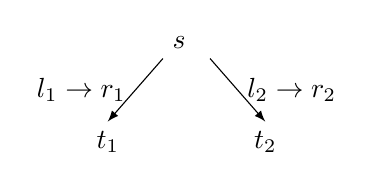
\begin{tikzpicture}
\draw [-latex] (0.7,0.8) node[above right] {$s$}-- node[left]{$l_1 \rightarrow r_1$} (0,0) node[below]{$t_1$} ;
\draw [-latex] (1.3,0.8) -- node[right]{$l_2 \rightarrow r_2$} (2,0) node[below]{$t_2$} ;
\end{tikzpicture}
\end{center}
La confluence locale sera assurée si nous trouvons un terme $t$ tel que 
$t_1 \overset{*}{\rightarrow} t \overset{*}{\leftarrow} t_2$ 

Nous avons ainsi 2 règles $l_1 \rightarrow r_1$ et $l_2 \rightarrow r_2$. Cela donne par définition de la réécriture :
$$ s|_{p_1} = \sigma_1 l_1\ avec\ t_1=s[\sigma_1 r_1]_{p_1} $$
$$ s|_{p_2} = \sigma_2 l_2\ avec\ t_2=s[\sigma_2 r_2]_{p_2} $$

On montre facilement (de manière visuelle) que nous pouvons trouver 
$t_1 \overset{*}{\rightarrow} t \overset{*}{\leftarrow} t_2$ lorsque
$p_1$ et $p_2$ ne se chevauchent pas. Et lorsqu'il y a chevauchement, on peut également trouver 
$t_1 \overset{*}{\rightarrow} t \overset{*}{\leftarrow} t_2$ si la position de $\sigma_2 l_2$ dans $l_1$ 
 est une variable.

\vspace{0.2cm}
Sinon, il y a un chevauchement \textit{critique} :
\begin{center}
	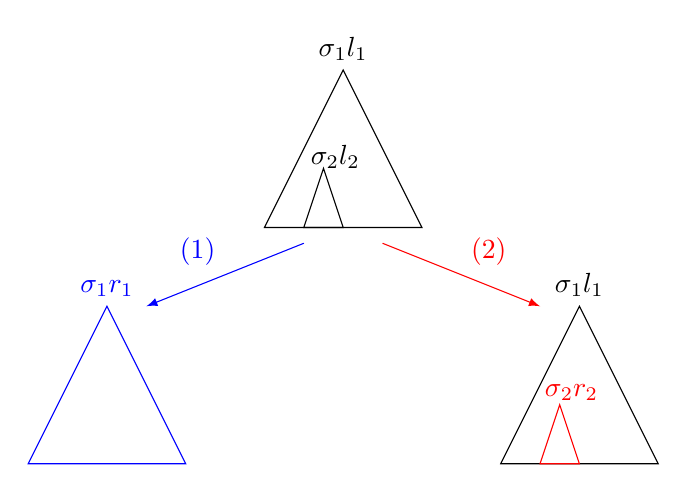
\begin{tikzpicture}
	\draw (0,0) -- (2,0) -- (1,2) node[above]{$\sigma_1 l_1$} --cycle ;
	\draw (0.5,0) --(1,0)-- (0.75,0.75)  --cycle ;
	\draw (0.9,0.9) node {$\sigma_2 l_2$} ;
	\draw [-latex, blue] (0.5,-0.2) -- node[above left] {$(1)$} (-1.5,-1) ;
	\draw [-latex, red] (1.5,-0.2) -- node[above right] {$(2)$} (3.5,-1) ;
	\begin{scope}[xshift=-3cm, yshift=-3cm]
		\draw [blue] (0,0) -- (2,0) -- (1,2) node[above]{$\sigma_1 r_1$} --cycle ;
	\end{scope}
	\begin{scope}[xshift=+3cm, yshift=-3cm] 
		\draw (0,0) -- (2,0) -- (1,2) node[above]{$\sigma_1 l_1$} --cycle ;
		\draw [red] (0.5,0) --(1,0)-- (0.75,0.75)  --cycle ;
		\draw [red] (0.9,0.9) node {$\sigma_2 r_2$} ;
	\end{scope}
	\end{tikzpicture}
	\end{center}

	Posons $\theta =  \sigma_1 \cup \sigma_2$, l'unificateur principal de $\sigma_1$ et $\sigma_2$.
	Nous appelerons la paire des deux termes en bleu et rouge
	 une \textit{paire critique} $<\theta r_1, (\theta l_1)[\theta r_2]_p > $
	 Si deux règles génèrent une paire critique, on dit qu'elles se superposent.
     L'existence de paires critiques est un signe d'ambiguïté du système de réécriture.

	 Si ces paires critiques sont joignable, le système de réécriture est alors localement confluent.
	 \begin{theoreme}[Knuth-Bendix]
		  Un système de réécriture noethérien est confluent si ses paires critiques sont joignables.
	\end{theoreme}
\begin{Verbatim}
let superpose l1 l2 =
let rec super l1 l2 occ =
	match occ with
	| a::b -> 
	begin
		try 
		let t = cut a l1 in
		match t with 
		| Var _ -> raise Impossible
		| _ -> let sigma = unifier ((cut a l1), l2)
				in (a, sigma)
		with Impossible -> super l1 l2 b 
	end
| [] -> raise Impossible
in super l1 l2 (occurences 0 l1)

let rec cp (l1,r1) (l2,r2) =
  let (oc, sigma) = superpose l1 l2 in
  ((substituer  r1 sigma), (greffe oc (substituer l1 sigma) (substituer r2 sigma))) ;;  
\end{Verbatim}


\subsection{Terminaison}
\subsubsection{Indécidabilité de la terminaison dans le cas "général"}
Soient $a_1,a_2 ,a_3 , \dots$ une numérotation de tous les algorithmes.
On définit la fonction suivante : $diag(i) ≡$ si $a_i$ termine alors \verb+boucler+, sinon \verb+s'arrêter+ \\

Pour tout $i$, $diag(i)$ termine ssi $a_i$ ne termine pas.
Mais il y a un $a_j$ tel que $diag = a_j$ . Nous avons donc
$diag(j)$ termine ssi $a_j$ ne termine pas, ce qui donne
$a_j$ termine ssi $a_j$ ne termine pas.


De manière peut-être plus formelle, en mettant en évidence la diagonalisation négative de Cantor :

Soit $f(x,y)$ la fonction de terminaison de l'algorithme $a_x$ sur l'entrée $y$.
On peut définir $f(x,y)$ comme $f(x,y) = 1$ si $a_x$ termine sur $y$ et $0$ sinon.
Soit $g$ telle que $g(0) = 1$ et $g(1) = 0$ 
Considérons $h(i) = g(f(i,i))$.
Alors on a $f(a,a) = h(a) = g(f(a,a)) \neq f(a,a)$ car $g$ n'admet pas de point fixe.
C'est-à-dire que l'on ne peut décider si l'algorithme $a_a$ termine sur lui-même. 

\vspace{0.5cm}

Cela donne en pseudo-code :
\begin{Verbatim}
halt(x) = si le programme x s'arrête alors vrai 
          sinon faux ;

diag(p) = si halt (p) alors boucle()
          sinon stop() ;
\end{Verbatim}
Quel est le comportement de \verb+halt(diag(diag))+ ?


S'il répond vrai, alors \verb+diag+ s'arrête alors qu'il est censé boucler par définition de \verb+diag+


S'il répond faux, alors \verb+diag+ boucle, alors qu'il est censé s'arrêter par défintion de \verb+diag+

\subsubsection{Système de réécriture noethérien}
Un système de réécriture est noethérien si et seulement s'il existe un ordre bien fondé
$\succ$ sur l'ensemble des termes tel que
\begin{itemize}
	\item[i)] $\sigma P \succ \sigma Q$ pour toute règle $(P,Q) \in \mathcal{R}$ et toute substitution $\sigma$
	\item[ii)] $M_i \succ M'_i$ entraîne $ fM_1\dots M_i \dots M_n \succ fM_1\dots M'_i \dots M_n $
\end{itemize}

On dit que $\succ$ est clos par substitution, et qu'il est compatible avec $\Sigma$.
\vspace{0.2cm}
En pratique, on utilise une fonction externe $h : T_\Sigma [X] \rightarrow \mathbb{N} $ et la relation d'ordre $>$ sur 
$\mathbb{N}$.

Pour un terme $t$ et une variable $x$ , on note $|t|$ le cardinal de $t$ et $|t|_x$ le nombre
d'occurrences de $x$ dans $t$. On définit un ordre strict $\succ$ sur $T[X]$ par :
$$ s > t \Leftrightarrow  |s| > |t|\ et\  \forall x \in X, |s|_x ≥ |t|_x $$

\subsection{Complétion de Knuth-Bendix}
Nous pourrons ici nous référer au livre très didactique \textit{Term Rewriting and All That}\cite{rewriting}
\begin{Verbatim}
let rec super_liste l1 l2 occ =
 match occ with
 | a::b -> 
	begin
	 try 
	 let t = cut a l1 in
	 match t with 
	 | Var _ -> raise Impossible
	 | _ -> let sigma = unifier ((cut a l1), l2)
 				in (a, sigma)
	 with Impossible -> super_liste l1 l2 b 
	 end
 | [] -> raise Impossible
  
let superpose_liste (l1,r1) (l2,r2) =
let rec superpose_liste_aux l1 l2 occ = (* rend liste des occurences et substitution *)
	if   alpha_equiv (l1,r1) (l2,r2) then 
		try
		let (oc, sigma) = super_liste l1 (rename l2 l1) (remove 0 occ) (* retire 0 car occurence triviale si alpha_equiv *)
		in 
		begin
			print_string "superposition à l'occurence "; print_int oc ;  print_string "\n" ;
			print_string "sur le termes l1 :" ; imprime l1 ; print_string "\n" ;
			print_string "sur le terme l2 :" ; imprime l2 ; print_string "\n" ;
			print_string "avec la substitution :"; imprime_sigma sigma; print_string "\n" ;
		(oc, sigma)::superpose_liste_aux l1 l2 (remove oc occ)
		end
		with Impossible -> []
	else 
	try
	let (oc, sigma) = super_liste l1 (rename l2 l1) occ
		in 
		begin print_string "superposition à l'occurence "; print_int oc ;  print_string "\n" ;
			print_string "sur le terme l1 :" ; imprime l1 ; print_string "\n" ;
			print_string "sur le terme l2 :" ; imprime l2 ; print_string "\n" ;
			print_string "avec la substitution :"; imprime_sigma sigma; print_string "\n" ;
			(oc, sigma)::superpose_liste_aux l1 l2 (remove oc occ)
		end
	with Impossible -> []
in superpose_liste_aux l1 l2 (occurences l1) ;;
\end{Verbatim}